% Options for packages loaded elsewhere
\PassOptionsToPackage{unicode}{hyperref}
\PassOptionsToPackage{hyphens}{url}
%
\documentclass[
]{article}
\usepackage{amsmath,amssymb}
\usepackage{iftex}
\ifPDFTeX
  \usepackage[T1]{fontenc}
  \usepackage[utf8]{inputenc}
  \usepackage{textcomp} % provide euro and other symbols
\else % if luatex or xetex
  \usepackage{unicode-math} % this also loads fontspec
  \defaultfontfeatures{Scale=MatchLowercase}
  \defaultfontfeatures[\rmfamily]{Ligatures=TeX,Scale=1}
\fi
\usepackage{lmodern}
\ifPDFTeX\else
  % xetex/luatex font selection
\fi
% Use upquote if available, for straight quotes in verbatim environments
\IfFileExists{upquote.sty}{\usepackage{upquote}}{}
\IfFileExists{microtype.sty}{% use microtype if available
  \usepackage[]{microtype}
  \UseMicrotypeSet[protrusion]{basicmath} % disable protrusion for tt fonts
}{}
\makeatletter
\@ifundefined{KOMAClassName}{% if non-KOMA class
  \IfFileExists{parskip.sty}{%
    \usepackage{parskip}
  }{% else
    \setlength{\parindent}{0pt}
    \setlength{\parskip}{6pt plus 2pt minus 1pt}}
}{% if KOMA class
  \KOMAoptions{parskip=half}}
\makeatother
\usepackage{xcolor}
\usepackage[margin=1in]{geometry}
\usepackage{longtable,booktabs,array}
\usepackage{calc} % for calculating minipage widths
% Correct order of tables after \paragraph or \subparagraph
\usepackage{etoolbox}
\makeatletter
\patchcmd\longtable{\par}{\if@noskipsec\mbox{}\fi\par}{}{}
\makeatother
% Allow footnotes in longtable head/foot
\IfFileExists{footnotehyper.sty}{\usepackage{footnotehyper}}{\usepackage{footnote}}
\makesavenoteenv{longtable}
\usepackage{graphicx}
\makeatletter
\def\maxwidth{\ifdim\Gin@nat@width>\linewidth\linewidth\else\Gin@nat@width\fi}
\def\maxheight{\ifdim\Gin@nat@height>\textheight\textheight\else\Gin@nat@height\fi}
\makeatother
% Scale images if necessary, so that they will not overflow the page
% margins by default, and it is still possible to overwrite the defaults
% using explicit options in \includegraphics[width, height, ...]{}
\setkeys{Gin}{width=\maxwidth,height=\maxheight,keepaspectratio}
% Set default figure placement to htbp
\makeatletter
\def\fps@figure{htbp}
\makeatother
\setlength{\emergencystretch}{3em} % prevent overfull lines
\providecommand{\tightlist}{%
  \setlength{\itemsep}{0pt}\setlength{\parskip}{0pt}}
\setcounter{secnumdepth}{-\maxdimen} % remove section numbering
\newlength{\cslhangindent}
\setlength{\cslhangindent}{1.5em}
\newlength{\csllabelwidth}
\setlength{\csllabelwidth}{3em}
\newlength{\cslentryspacingunit} % times entry-spacing
\setlength{\cslentryspacingunit}{\parskip}
\newenvironment{CSLReferences}[2] % #1 hanging-ident, #2 entry spacing
 {% don't indent paragraphs
  \setlength{\parindent}{0pt}
  % turn on hanging indent if param 1 is 1
  \ifodd #1
  \let\oldpar\par
  \def\par{\hangindent=\cslhangindent\oldpar}
  \fi
  % set entry spacing
  \setlength{\parskip}{#2\cslentryspacingunit}
 }%
 {}
\usepackage{calc}
\newcommand{\CSLBlock}[1]{#1\hfill\break}
\newcommand{\CSLLeftMargin}[1]{\parbox[t]{\csllabelwidth}{#1}}
\newcommand{\CSLRightInline}[1]{\parbox[t]{\linewidth - \csllabelwidth}{#1}\break}
\newcommand{\CSLIndent}[1]{\hspace{\cslhangindent}#1}
\ifLuaTeX
  \usepackage{selnolig}  % disable illegal ligatures
\fi
\IfFileExists{bookmark.sty}{\usepackage{bookmark}}{\usepackage{hyperref}}
\IfFileExists{xurl.sty}{\usepackage{xurl}}{} % add URL line breaks if available
\urlstyle{same}
\hypersetup{
  pdftitle={Analysis of staffing levels for nursing and adult inpatient care},
  pdfauthor={Mairead Bermingham},
  hidelinks,
  pdfcreator={LaTeX via pandoc}}

\title{Analysis of staffing levels for nursing and adult inpatient care}
\author{Mairead Bermingham}
\date{2023-08-10}

\begin{document}
\maketitle

\hypertarget{scenario}{%
\section{Scenario}\label{scenario}}

Job applicants have been asked as part of the interview process for the
`Data and Measurement Advisory' role with Healthcare Improvement
Scotland (HIS) have been asked to analyse staffing levels data across
three Clinical areas collected daily by the Senior Charge Nurse, and to
present and discuss finding at hospital management meeting to discuss
safe staffing levels within Hospital X. Clinical area A and B are 25 and
30 bedded adult inpatient wards respectively. Bed capacity can be over
100\% due to admissions/discharges and the opening of surge beds where
available. All data, charts, images, documents and code associated with
this exercise can be accessed from
\href{https://github.com/MaireadLBermingham/Staffing_levels_for_Nursing_and_Adult_Inpatient_Care_Quality_and_Safety.git}{gitHub}

\hypertarget{aim}{%
\section{Aim}\label{aim}}

\hypertarget{health-and-care-staffing-scotland-act-2019}{%
\subsection{Health and Care (Staffing) (Scotland) Act
2019}\label{health-and-care-staffing-scotland-act-2019}}

The Act was passed by the Scottish Parliament in 2019. Its
implementation was paused due to the COVID-19 pandemic. All the
provisions within the Act will come into force in April 2024. The Act
was passed by Parliament in 2019, but implementation was paused due to
the pandemic. All the provisions within the Act will come into force in
April 2024. The aim of the Act is to be an enabler of high-quality care
and improved outcomes for service users of health service and care
services by ensuring appropriate staffing.

\hypertarget{general-duty}{%
\subsubsection{General duty}\label{general-duty}}

The Act places duties on health boards, care service providers,
Healthcare Improvement Scotland (HIS), the Care Inspectorate and
Scottish Ministers. to ensure appropriate staffing. As health
professionals, it is our duty to ensuring both appropriate numbers and
types of staff as necessary are working as appropriate for\\
* health, welling and safety of patients\\
* and provision of safe and high-quality care * staff well-being in so
far as it impacts the aforementioned conditions.\\
We are also required to submit quarterly Board reports, and to publish
and submit an annual report to the Scottish Ministers detailing how it
has carried out its duties under the following sections

Our \textbf{aim} is to ensure safe and high-quality care through
consistent data collection to scaffold improvement initiatives, and
facilitate mandatory reporting, maintain the proportion of registered
nurses as a percentage of total nursing staff above 65\%, and the whole
time equivalent (WTE) used meets or exceeds the WTE required to staff
the ward.

\hypertarget{adult-inpatient-care-journey}{%
\subsection{Adult inpatient care
journey}\label{adult-inpatient-care-journey}}

The patient will be referred by a GP or Accident and emergency service,
and will be admitted from outpatients or theater to the inpatient ward,
where a nurse will look after them and manage their pain. The patient
will be cared for by the healthcare team, which includes doctors,
nurses, healthcare assistants and others. Staff on the wards will be
working to a planned date for their discharge home or into community
care (Figure 1).

\begin{figure}
\centering
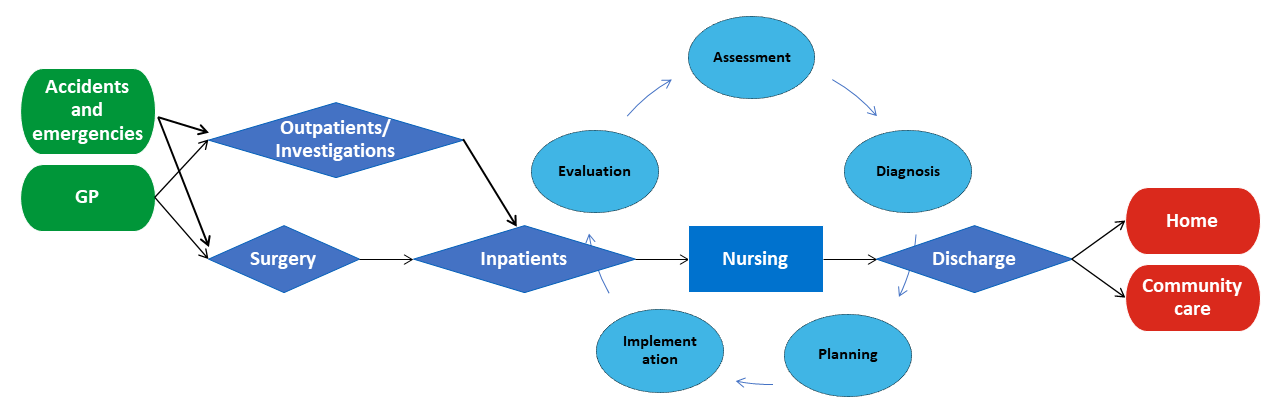
\includegraphics{./../../Output/Visuals/Adult inpatient care journey.png}
\caption{Figure 1. The adult inpatient care journey. This figure shows
is the steps in reviewing and developing a nursing care plan for adult
inpatients addmitted onto an inpatient ward.}
\end{figure}

\hypertarget{the-nursing-process}{%
\subsection{The nursing process}\label{the-nursing-process}}

The nursing process is a methodical problem-solving approach used to
identify, prevent and treat actual or potential health issues and
promote well-being. It has five steps: assessment, diagnosis, planning,
implementation and evaluation (Figure 2)
(\protect\hyperlink{ref-semachew2018ImplementationNursingProcess}{Semachew,
2018}).

\begin{figure}
\centering
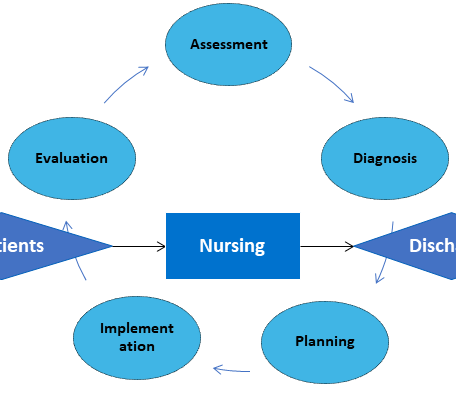
\includegraphics{./../../Output/Visuals/Adult inpatient care journey_Nursing.png}
\caption{Figure 2. The nursing process. This figure focuses on the five
steps in nursing of adult inpatients addmitted onto an inpatient ward
process.}
\end{figure}

\hypertarget{dma-data}{%
\subsubsection{DMA data}\label{dma-data}}

The data provided as part of the Data and Measurement Advisory job
interview process will collected by a Senior staff nurse and her line
manager and team from Clinical areas, using the Professional Judgement
and Adult In-Patient tools. The tools are applied concurrently for at
least 2 weeks (14 consecutive days, with no intervening days)
(\protect\hyperlink{ref-healthcareimprovementscotland2022AdultInpatientWorkload}{Scotland,
2022}).

\hypertarget{the-professional-judgement-tool}{%
\paragraph{The Professional Judgement
tool}\label{the-professional-judgement-tool}}

The Professional Judgement tool facilitates compliance with national
recommendations that Senior staff nurses and their line managers should
use this tool to determine staffing requirements, supporting an
evidence-based workforce planning.

\hypertarget{adult-in-patient}{%
\paragraph{Adult In-Patient}\label{adult-in-patient}}

The Adult In-Patient tool supports Senior staff nurses and their line
managers in making evidence‐based staffing levels decisions by assessing
patient dependency and/or acuity and nursing activity.

\hypertarget{process-measures}{%
\paragraph{Process measures}\label{process-measures}}

\hypertarget{measures-that-indicate-that-steps-we-have-put-in-place-to-achive-our-stated-aim-are-being-reliably-implemented.}{%
\paragraph{Measures that indicate that steps we have put in place to
achive our stated aim are being reliably
implemented.}\label{measures-that-indicate-that-steps-we-have-put-in-place-to-achive-our-stated-aim-are-being-reliably-implemented.}}

The data provided by the recruitment panel consists of a serious of
process measures of available staff, and patient care complexity data
(Table 1).

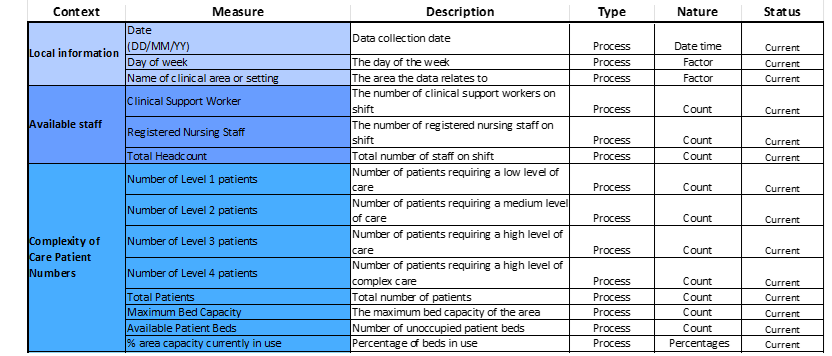
\includegraphics{./../../Output/Visuals/DataDictionary.png} \#\#\#\#
Measures of nursing care quality and performance However measures of
nursing care quality and performance across the Nursing process are not
included in the DMA data (Figure 2). I would like to propose to the
Senior staff nurse during the management meeting that we should be
making use of routinely collected nursing sensitive indicators to
determine whether nursing care quality and performance has an impact
patients (Table 2)
(\protect\hyperlink{ref-oner2021NursingSensitiveIndicators}{Oner et al.,
2021}).

\begin{figure}
\centering
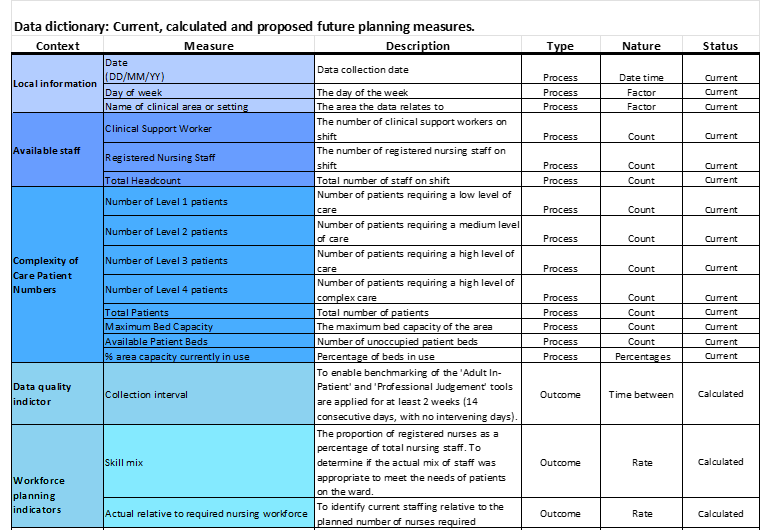
\includegraphics{./../../Output/Visuals/UpdatedDataDictionary.png}
\caption{Table 2. Updated DMA data dictionary. This table provides
descripts of the context, descrition, type and nature of the DMA data
pata provied by the recruitment panel, calculated and posposed
measures.}
\end{figure}

\hypertarget{outcome-measures}{%
\paragraph{Outcome measures}\label{outcome-measures}}

\hypertarget{measures-that-demonstrate-or-not-that-we-are-working-toward-achiveng-our-stated-aim.}{%
\subparagraph{Measures that demonstrate or not that we are working
toward achiveng our stated
aim.}\label{measures-that-demonstrate-or-not-that-we-are-working-toward-achiveng-our-stated-aim.}}

There are no outcome measures included in the DMA data that directly
more improved performance or that we are working towards or stated aim
of ensuring safe and high quality care through \textbf{consistent data
collection} to scaffold improvement initiatives, and facile an mandatory
reporting, maintain the \textbf{proportion of registered nurses as
percentage of total nursing staff above 65\%}, and the \textbf{whole
time equivalent (WTE) used meets or exceeds the WTE required} to staff
the ward. I have there for used the process measures provided to
calculate three outcomes measures: * \textbf{Collection interval.} To
enable benchmarking, the Adult In-Patient and Professional Judgement
tools are applied for at least 2 weeks (14 consecutive days, with no
intervening days). * \textbf{Proportion of registered nurses (RN) as
percentage of total nursing staff.} To determine if the actual mix of
staff was appropriate to meet the needs of patients on the ward. The
benchmark average on general hospital wards is 65\% registered nurses
(Table 2)
(\protect\hyperlink{ref-royalcollegeofnursingRCNPolicyUnit2006}{Nursing,
2006}).

\hypertarget{balancing-measures}{%
\paragraph{Balancing measures}\label{balancing-measures}}

\hypertarget{measures-that-track-if-improvements-in-one-part-of-the-system-to-ensure-they-are-causing-unintended-consequences-elsewhere-in-the-system.}{%
\subparagraph{Measures that track if improvements in one part of the
system to ensure they are causing unintended consequences elsewhere in
the
system.}\label{measures-that-track-if-improvements-in-one-part-of-the-system-to-ensure-they-are-causing-unintended-consequences-elsewhere-in-the-system.}}

We need to look at the systems as a whole from different directions and
ensure that staffing improvements not causing problems in other parts of
the system. I would like to propose to the Senior staff nurse during the
management meeting that we should be making use of the routinely
collected staff turnover, sickness absence and agency spend balancing
measures to reflect what may be happening elsewhere in the system as a
result of the staffing improvements in the adult inpatient ward (Table
2) (\protect\hyperlink{ref-ball2010GuidanceSafeNurse}{Ball, 2010}).

\hypertarget{updating-the-dma-exercise-data}{%
\section{Updating the DMA Exercise
data}\label{updating-the-dma-exercise-data}}

I develop accessible, transparent, time saving, data and measurement
handing pipelines, exploratory and downstream analyses and reports in
RMarkdown, and use GitHub version control to make it possible for
others, including my future self, to collaborate on projects and
reproduce results. Many stakeholder are not familiar with R nor
accessing project folder and documents via GitHub. I there for produce
less technical, code free reports, MS Excel Workbooks and PowerPoint
presentations as part of my workflow to facilitate collaboration with
less technical stakeholders.

Table 1. DMA Exercise data structure.

\begin{verbatim}
## tibble [54 x 14] (S3: tbl_df/tbl/data.frame)
##  $ Date                      : POSIXct[1:54], format: "2023-01-01" "2023-01-01" ...
##  $ Day                       : chr [1:54] "Sunday" "Sunday" "Monday" "Monday" ...
##  $ ClinicalArea              : chr [1:54] "B" "A" "B" "A" ...
##  $ Clinical Support Worker   : num [1:54] 4 3 3 2 4 3 4 2 4 4 ...
##  $ Registered Nursing Staff  : num [1:54] 5 3 3 3 6 4 3 3 3 4 ...
##  $ Total Headcount           : logi [1:54] NA NA NA NA NA NA ...
##  $ Number of Level 1 patients: num [1:54] 10 12 8 9 14 14 10 11 10 11 ...
##  $ Number of Level 2 patients: num [1:54] 7 7 6 5 9 7 8 6 8 9 ...
##  $ Number of Level 3 patients: num [1:54] 4 3 2 5 6 5 4 3 4 4 ...
##  $ Number of Level 4 patients: num [1:54] 3 2 1 3 4 2 1 2 1 3 ...
##  $ Total Patients            : logi [1:54] NA NA NA NA NA NA ...
##  $ Maximum Bed Capacity      : logi [1:54] NA NA NA NA NA NA ...
##  $ Available Patient Beds    : logi [1:54] NA NA NA NA NA NA ...
##  $ Activity                  : logi [1:54] NA NA NA NA NA NA ...
\end{verbatim}

The data fame included 14 variables and 54 rows. The `Day of
week',`Total Headcount', `Total Patients', `Maximum Bed
Capacity',`Available Patient Beds', and `\% area capacity currently in
use (Total Patients/Maximum Bed Capacity)' variables are empty and need
to be populated.

\hypertarget{populating-the-total-headcount-total-patients-maximum-bed-capacity-available-patient-beds-and-area-capacity-currently-in-use-process-measures.}{%
\subsection{Populating the `Total Headcount' , `Total Patients',
`Maximum Bed Capacity', `Available Patient Beds' and `\% area capacity
currently in use' process
measures.}\label{populating-the-total-headcount-total-patients-maximum-bed-capacity-available-patient-beds-and-area-capacity-currently-in-use-process-measures.}}

In the `Scenario tab in the DMA Exercise data MS Excel file we were
informed that Clinical area A is a 25 bedded ward, and Clinical area B
is a 30 bedded ward. Furthermore we were told that bed capacity can be
over 100\% due to admissions/discharges and opening of surge beds where
available. This information was used information to populated the
'Maximum Bed Capacity' variable.

\begin{verbatim}
## # A tibble: 6 x 14
##   Date                Day     ClinicalArea `Clinical Support Worker`
##   <dttm>              <chr>   <chr>                            <dbl>
## 1 2023-01-01 00:00:00 Sunday  B                                    4
## 2 2023-01-01 00:00:00 Sunday  A                                    3
## 3 2023-01-02 00:00:00 Monday  B                                    3
## 4 2023-01-02 00:00:00 Monday  A                                    2
## 5 2023-01-03 00:00:00 Tuesday B                                    4
## 6 2023-01-03 00:00:00 Tuesday A                                    3
## # i 10 more variables: `Registered Nursing Staff` <dbl>,
## #   `Total Headcount` <dbl>, `Number of Level 1 patients` <dbl>,
## #   `Number of Level 2 patients` <dbl>, `Number of Level 3 patients` <dbl>,
## #   `Number of Level 4 patients` <dbl>, `Total Patients` <dbl>,
## #   `Maximum Bed Capacity` <dbl>, `Available Patient Beds` <dbl>,
## #   `% area capacity currently in use` <dbl>
\end{verbatim}

\hypertarget{populating-the-day-of-the-week-variable}{%
\subsection{Populating the day of the week
variable}\label{populating-the-day-of-the-week-variable}}

I use the `lubricate' package to extract the day of the week from the
Date variable. `Lubridate' is an R package that makes it easier to work
with dates and times.

\hypertarget{looking-at-the-consistentancy-of-collection-across-week-days.}{%
\subsubsection{Looking at the consistentancy of collection across week
days.}\label{looking-at-the-consistentancy-of-collection-across-week-days.}}

Table 1. Frequency distribution of day of the week by Clinical area.

\begin{verbatim}
## # A tibble: 3 x 8
##   ClinicalArea   Mon   Tue   Wed   Thu   Fri   Sat   Sun
##   <chr>        <int> <int> <int> <int> <int> <int> <int>
## 1 A                4     3     4     1     3     4     4
## 2 B                5     5     1     4     4     4     5
## 3 C                0     0     1     0     1     0     1
\end{verbatim}

Consistency of collection appears greater in Clinical area B based on
the frequency distribution of day of the week. There appears at first
glance to be a relationship between low week day counts in Clinical area
A and data collected in Clinical area A. Could it be that the team
misassigned the name of the clinical area.

\hypertarget{examining-the-relationship-between-the-dates-data-was-collected-in-clinical-area-c-and-the-other-two-areas.}{%
\section{Examining the relationship between the dates data was collected
in Clinical area C and the other two
areas.}\label{examining-the-relationship-between-the-dates-data-was-collected-in-clinical-area-c-and-the-other-two-areas.}}

There is only one of the three dates, the 11/1/2023 that you could infer
the the team may have misassigned the name of Clinical area B with C.
Before making this change, I would have to confirm this with the Senior
Charge Nurse. For the purpose, of the analyses for the upcoming meeting,
I will assume the data has been correctly assassinated to Clinical area
C. Data was collected at all three Clinical areas for the other two
dates.

\hypertarget{clinical-area-c}{%
\paragraph{Clinical area C}\label{clinical-area-c}}

Ward capacity details were not provided for Clinical area C. As such the
`\% area capacity currently in use' measure can not be calculated. Only
Clinical area A and B will be included in down stream analysis, and the
last three records in the data set from Clinical area C removed.

\hypertarget{calculating-the-the-collection-interval-skill-mix-and-nurse-staffing-relative-to-patient-requirments-outcome-measures}{%
\subsection{Calculating the the `Collection interval', `Skill mix' and
`Nurse staffing relative to patient requirments' outcome
measures}\label{calculating-the-the-collection-interval-skill-mix-and-nurse-staffing-relative-to-patient-requirments-outcome-measures}}

\hypertarget{exmaming-the-consistance-of-data-collection-in-cinical-areas-a-and-b.}{%
\paragraph{Exmaming the consistance of data collection in Cinical areas
A and
B.}\label{exmaming-the-consistance-of-data-collection-in-cinical-areas-a-and-b.}}

To determine the consistency of data collection I calculated the data
collection interval.

Table 1. The frequency distribution of Collection interval by Clinical
Area.

\begin{longtable}[]{@{}lrrr@{}}
\toprule\noalign{}
Clinical area & Collection interval & Frequency & Percent \\
\midrule\noalign{}
\endhead
\bottomrule\noalign{}
\endlastfoot
A & 1 & 15 & 68.18\% \\
A & 2 & 6 & 27.27\% \\
A & 3 & 1 & 4.55\% \\
B & 1 & 24 & 88.89\% \\
B & 2 & 3 & 11.11\% \\
\end{longtable}

The consistency of data collection was much higher in Clinical area B,
compared to A. In total, 89\% of records were collected within one data,
as opposed to 68\% in clinical area C.

\hypertarget{calculating-the-skill-mix-and-nurse-staffing-relative-to-patient-requirements-outcome-varaiables}{%
\subsubsection{Calculating the `Skill mix' and Nurse staffing relative
to patient requirements outcome
varaiables}\label{calculating-the-skill-mix-and-nurse-staffing-relative-to-patient-requirements-outcome-varaiables}}

Skill mix was simply calculated as the rate of Registered nursing staff
to total nursing staff. !

\begin{figure}
\centering
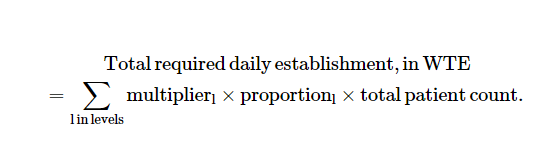
\includegraphics{./../../Output/Visuals/rWTE.png}
\caption{The total daily required establishment, WTE was calculated as.}
\end{figure}

Using general ward multipliers for level 1-4 patients
(\protect\hyperlink{ref-griffiths2020SaferNursingCare}{Griffiths et al.,
2020}).

\begin{verbatim}
## < table of extent 0 >
\end{verbatim}

\hypertarget{checking-for-missing-records-and-removing-redundant-variables}{%
\section{Checking for missing records and removing redundant
variables}\label{checking-for-missing-records-and-removing-redundant-variables}}

\begin{longtable}[]{@{}rrr@{}}
\toprule\noalign{}
lag1\_Date & lag1\_ClinicalArea & CollectionInterval \\
\midrule\noalign{}
\endhead
\bottomrule\noalign{}
\endlastfoot
2 & 2 & 2 \\
\end{longtable}

The data is complete, the only missing records are those associated with
the `Collection interval' measure. I have set those missing records to
zero, and removed redundant variables.

\hypertarget{adding-the-updated-data-to-the-dma-exercise-data-excel-file}{%
\section{Adding the updated data to the DMA Exercise data Excel
file}\label{adding-the-updated-data-to-the-dma-exercise-data-excel-file}}

The original DMA Exercise data Excel file was read in again, and a
working DMA Exercise working data Excel file set up in the project
output data folder to collect, data updates, summary tables, charts,
results and comments for stakeholder to review prior to the Hospital X
management meeting.

\hypertarget{visual-representation-of-the-three-calculated-outcome-variables}{%
\section{Visual representation of the three calculated outcome
variables}\label{visual-representation-of-the-three-calculated-outcome-variables}}

\begin{verbatim}
## [1] "We have 23 and 28 data points in Clinical areas A and B respectively. This means the lower limit for the number of runs are seven and ten and the upper limit is 17 and 20 runs to demonstrate non-random variable attributable to changes in staffing levels."
\end{verbatim}

\includegraphics{Analysis_of_staffing_levels_for_nursing_and_adult_inpatient_care_files/figure-latex/Runcharts-1.pdf}

\begin{verbatim}
## [1] "The collection interval for Clinical area A was inconsistent. No shifts or trends were seen on the run chart. The median was one, it was therefore not possible to assess the number of runs. However, an astronomical point of three days was measured on Saturday the 14th of January 2023."
\end{verbatim}

\includegraphics{Analysis_of_staffing_levels_for_nursing_and_adult_inpatient_care_files/figure-latex/Runcharts-2.pdf}

\begin{verbatim}
## [1] "The collection interval for Clinical area C was more consistent, only missing three sample dates. No shifts or trends were seen on the run chart. Six runs can be seen on the run chant, which is below the lower limit of 10, suggesting statistically significant change."
\end{verbatim}

\includegraphics{Analysis_of_staffing_levels_for_nursing_and_adult_inpatient_care_files/figure-latex/Runcharts-3.pdf}

\begin{verbatim}
## [1] "The Skill mix for Clinical area A was low and variable and only exceeded the benchmark of .65 on Thursday, the 19th of January 2023. No shifts or trends were seen on the run chart. Thirteen runs can be seen on the run chant, which is below the upper limit of 17, suggesting no statistically significant change. However, an astronomical point of .33 was measured on Sunday the 22nd of January 2023."
\end{verbatim}

\includegraphics{Analysis_of_staffing_levels_for_nursing_and_adult_inpatient_care_files/figure-latex/Runcharts-4.pdf}

\begin{verbatim}
## [1] "The Skill mix for Clinical area B was also low and variable and only exceeded the benchmark of .65 on Thursday, the 12th and 19th of January 2023. Clinical area A also exceeded the benchmark on the 19th of January, 2023. It was interesting to hear what insights Senior Charge Nurse has as to why performance improved dramatically at the two Clinical areas on that date.  No shifts or trends were seen on the run chart. Eighteen runs can be seen on the run chant, which is below the upper limit of 20, suggesting no statistically significant change. However, an astronomical point of .33 was measured on Sunday the 29th of January 2023."
\end{verbatim}

\includegraphics{Analysis_of_staffing_levels_for_nursing_and_adult_inpatient_care_files/figure-latex/Runcharts-5.pdf}

\begin{verbatim}
## [1] "The Actual relative to required nursing Workforce for Clinical area A fell below our set benchmark of one on six occasions.  No shifts or trends were seen on the run chart. Eleven runs can be seen on the run chant, which is below the upper limit of 20, suggesting no statistically significant change. However, an astronomical point of 1.62 was measured on Sunday the 22nd of January 2023."
\end{verbatim}

\includegraphics{Analysis_of_staffing_levels_for_nursing_and_adult_inpatient_care_files/figure-latex/Runcharts-6.pdf}

\begin{verbatim}
## [1] "The Actual relative to required nursing Workforce for Clinical area B fell below our set benchmark of one on nine occasions.  No shifts or trends were seen on the run chart. Eleven runs can be seen on the run chant, which is above the lower limit of 10, suggesting no statistically significant change. However, astronomical points of 1.79 and 1.76 were measured on Monday the 9th and Sunday the 29th of January 2023. Another astronomical point of 0.65 was measured on the 31st of January, 2023."
\end{verbatim}

\hypertarget{references}{%
\section*{References}\label{references}}
\addcontentsline{toc}{section}{References}

\hypertarget{refs}{}
\begin{CSLReferences}{1}{0}
\leavevmode\vadjust pre{\hypertarget{ref-ball2010GuidanceSafeNurse}{}}%
Ball, J., 2010.
\href{https://www.rcn.org.uk/-/media/Royal-College-Of-Nursing/Documents/Publications/Obselete/PUB-003860.pdf}{Guidance
on safe nurse staffing levels in the {UK}}.

\leavevmode\vadjust pre{\hypertarget{ref-griffiths2020SaferNursingCare}{}}%
Griffiths, P., Saville, C., Ball, J.E., Chable, R., Dimech, A., Jones,
J., Jeffrey, Y., Pattison, N., Saucedo, A.R., Sinden, N., 2020. The
{Safer} {Nursing} {Care} {Tool} as a guide to nurse staffing
requirements on hospital wards: Observational and modelling study.

\leavevmode\vadjust pre{\hypertarget{ref-royalcollegeofnursingRCNPolicyUnit2006}{}}%
Nursing, R.C. of, 2006.
\href{https://www.rcn.org.uk/-/media/Royal-College-Of-Nursing/Documents/Policies-and-briefings/UK-Wide/Policies/2006/1506.pdf}{{RCN}
policy unit policy guidance 15/2006: Setting appropriate ward nurse
staffing levels in {NHS} acute trusts}.

\leavevmode\vadjust pre{\hypertarget{ref-oner2021NursingSensitiveIndicators}{}}%
Oner, B., Zengul, F.D., Oner, N., Ivankova, N.V., Karadag, A.,
Patrician, P.A., 2021. Nursing‐sensitive indicators for nursing care:
{A} systematic review (1997--2017). Nursing open 8, 1005--1022.

\leavevmode\vadjust pre{\hypertarget{ref-healthcareimprovementscotland2022AdultInpatientWorkload}{}}%
Scotland, H.I., 2022.
\href{https://www.healthcareimprovementscotland.org/idoc.ashx?docid=d6d8c442-ccc1-4eac-a3b3-98efe55df4e5\&version=-1}{Adult
inpatient workload tool: {User} guide}.

\leavevmode\vadjust pre{\hypertarget{ref-semachew2018ImplementationNursingProcess}{}}%
Semachew, A., 2018. Implementation of nursing process in clinical
settings: The case of three governmental hospitals in {Ethiopia}, 2017.
BMC research notes 11, 1--5.

\end{CSLReferences}

\end{document}
